\documentclass{beamer}
\usepackage[utf8]{inputenc}

\usetheme{Madrid}
\usecolortheme{default}

\usepackage{amsmath,amssymb}
\usepackage{txfonts}
\usepackage{tikz}
\usepackage{graphicx}
\usepackage{listings}
\usepackage{adjustbox}
\usepackage{array}
\usepackage{tabularx}
\usepackage{gvv}   % for \myvec command

% ---------- listings setup (works on Overleaf Free) ----------
\usepackage{xcolor}
\lstset{
  basicstyle=\ttfamily\small,
  keywordstyle=\color{blue},
  commentstyle=\color{gray},
  stringstyle=\color{red},
  breaklines=true,
  showstringspaces=false,
  numbers=left,
  numberstyle=\tiny,
  frame=single,
  tabsize=2
}
% -------------------------------------------------------------

% Title info
\title{MatGeo Assignment}
\subtitle{Problem 1.2.15}
\author{AI25BTECH11009 -- Dasu Harshith Kumar}
\date{\today}

\begin{document}

% Title Slide
\begin{frame}
  \titlepage
\end{frame}

% Question
\begin{frame}{Question 1.2.15}
Verify if the points  
\[
A(4,3), \; B(6,4), \; C(5,-6), \; D(-3,5)
\]  
are the vertices of a parallelogram.
\end{frame}

% Theoretical Solution 1
\begin{frame}{Theoretical Solution}
A quadrilateral is a parallelogram if the diagonals bisect each other,
i.e., the midpoints of $AC$ and $BD$ are the same.

Midpoint of diagonal $AC$:
\[
M_{AC}=\frac{A+C}{2}
=\frac{1}{2}\myvec{4+5\\3+(-6)}
=\myvec{4.5\\-1.5}
\]
\end{frame}

% Theoretical Solution 2
\begin{frame}{Theoretical Solution}
Midpoint of diagonal $BD$:
\[
M_{BD}=\frac{B+D}{2}
=\frac{1}{2}\myvec{6+(-3)\\4+5}
=\myvec{1.5\\4.5}
\]

Since $M_{AC}\neq M_{BD}$, the diagonals do not bisect each other.
\[
\therefore\; A,B, C, D \text{ do not form a parallelogram.}
\]
\end{frame}

% ---------------- C CODE (split across two slides) ----------------
\begin{frame}[fragile]{C Code - Midpoint of diagonals}
\begin{lstlisting}[language=C]
// midpoint.c (part 1/2)
#include <stdio.h>

void midpoint(double x1, double y1, double x2, double y2,
              double* mx, double* my) {
    *mx = (x1 + x2) / 2.0;
    *my = (y1 + y2) / 2.0;
}

int main() {
    double mx, my;

    // AC midpoint
    midpoint(4, 3, 5, -6, &mx, &my);
    printf("Midpoint AC = (%lf, %lf)\n", mx, my);
\end{lstlisting}
\end{frame}

\begin{frame}[fragile]{C Code - Midpoint of diagonals (cont.)}
\begin{lstlisting}[language=C]
// midpoint.c (part 2/2)

// BD midpoint
midpoint(6, 4, -3, 5, &mx, &my);
printf("Midpoint BD = (%lf, %lf)\n", mx, my);

return 0;
}
\end{lstlisting}
\end{frame}
% ------------------------------------------------------------------

% --------------- PYTHON CODE (split across two slides) -------------
\begin{frame}[fragile]{Python Code}
\begin{lstlisting}[language=Python]
# plot_parallelogram_check.py (part 1/2)
import matplotlib.pyplot as plt

A = (4, 3)
B = (6, 4)
C = (5, -6)
D = (-3, 5)

# Midpoints
M_AC = ((A[0]+C[0])/2, (A[1]+C[1])/2)
M_BD = ((B[0]+D[0])/2, (B[1]+D[1])/2)

print("Midpoint AC =", M_AC)
print("Midpoint BD =", M_BD)
\end{lstlisting}
\end{frame}

\begin{frame}[fragile]{Python Code (cont.)}
\begin{lstlisting}[language=Python]
# plot_parallelogram_check.py (part 2/2)
plt.figure(figsize=(6,6))
x = [A[0], B[0], C[0], D[0], A[0]]
y = [A[1], B[1], C[1], D[1], A[1]]
plt.plot(x, y, 'ro-')

for P, name in zip([A,B,C,D,M_AC,M_BD],
                   ['A','B','C','D','M_AC','M_BD']):
    plt.text(P[0]+0.2, P[1]+0.2, name, fontsize=10)

plt.grid(True)
plt.gca().set_aspect('equal', adjustable='box')
plt.title("Check if ABCD is a Parallelogram")

# Save (optional) and/or show
plt.savefig("figs/1_2_15.jpg", dpi=300, bbox_inches="tight")
plt.show()
\end{lstlisting}
\end{frame}
% ------------------------------------------------------------------

% Plot slide
\begin{frame}{Plot}
\centering
% Put 1_2_15.png in the figs/ folder of your project
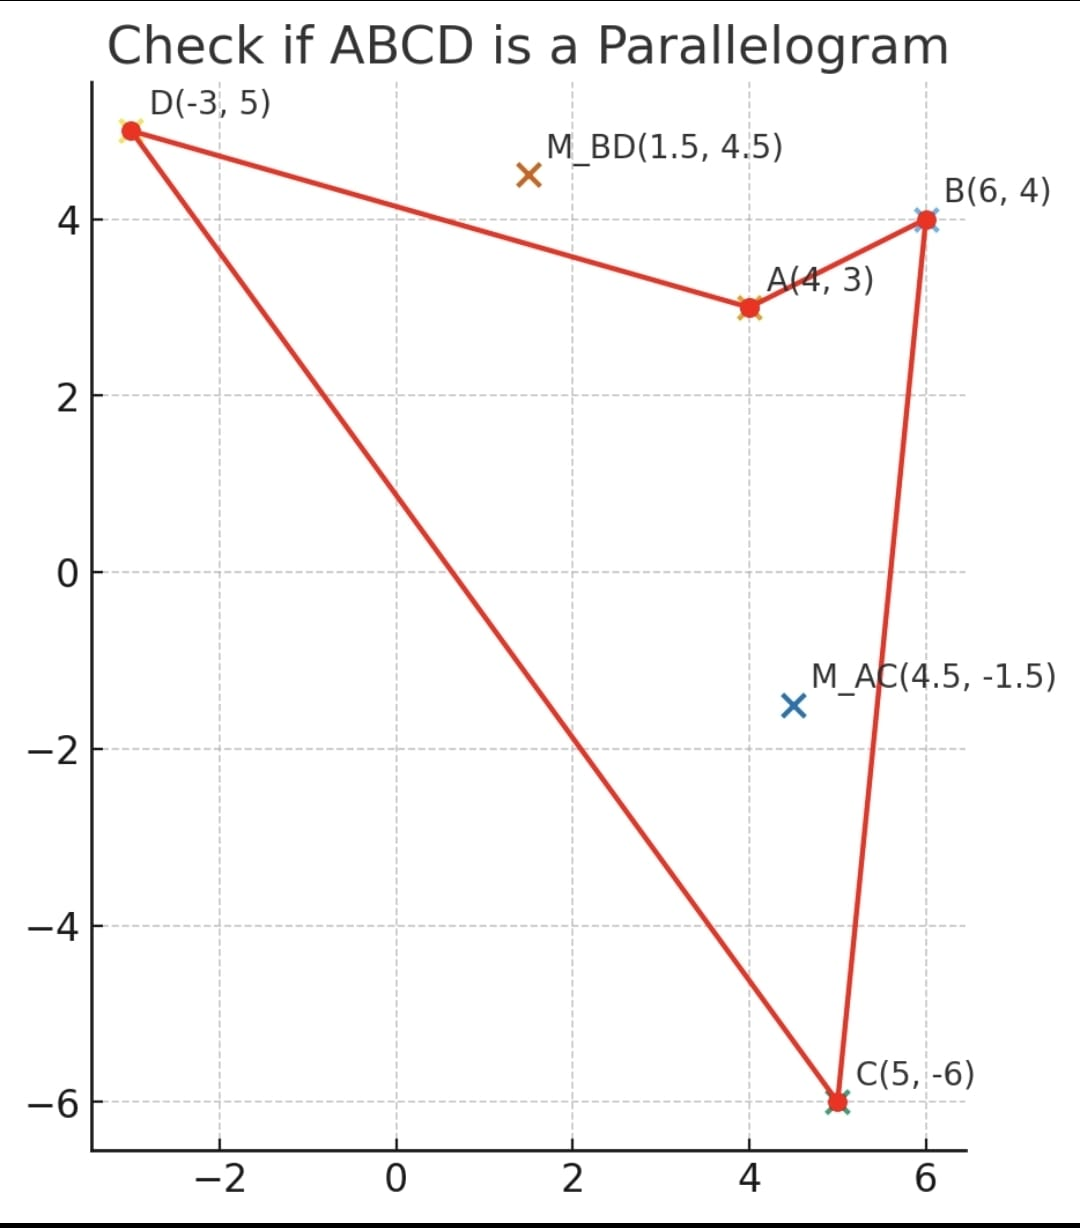
\includegraphics[width=0.61\linewidth]{figs/1_2_15.jpg}
\end{frame}

\end{document}
